\section{ADC}
The digital logic used to determine the colour of a brick requires that the analog voltage is converted to a digital value. To this end, an analog to digital converter, ADC, is used. Specifically an MCP3008 \cite{mcp3008} which is a 10 bit ADC.
\subsection{The ADC: MCP3008}
As mentioned, the MCP3008 is an ADC, it is capable of converting an analog value ranging from 0 to V$_{\text{ref}}$ into a 10 bit value. It is rated to have a conversion rate of 200 ksps at V$_{\text{dd}} = 5$V. 

\begin{figure}[h!]
	\begin{subfigure}[b]{.48\linewidth}
		\centering
		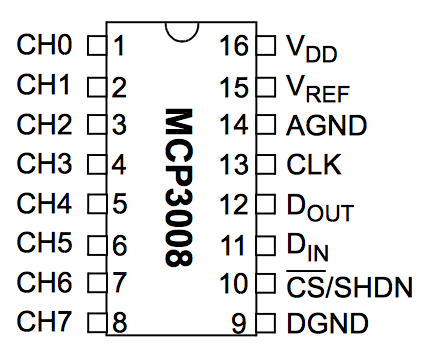
\includegraphics[width=.5\linewidth]{images/MPC3008.png}
		\caption{Pinout diagram of the MCP3008 ADC.}
		\label{fig:pinout}
	\end{subfigure}
	\begin{subfigure}[b]{.48\linewidth}
		\centering
		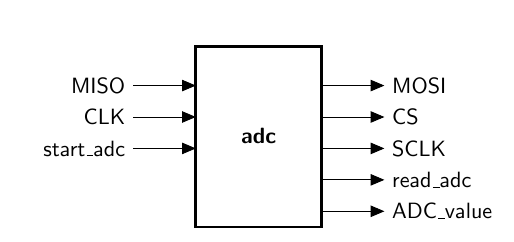
\includegraphics[width=\linewidth]{images/ADC_ent}
		\caption{The ADC component pinout}
		\label{fig:adcpinout}
	\end{subfigure}
\end{figure}
As can be seen on figure \ref{fig:pinout}, The chip is a 16 pin dip package. Pins 1 through 8 consist of eight seperate input ports for analog voltages. Pins 9 through 16 are, in descending order: V\textsubscript{dd}, V\textsubscript{ref}, AGND , CLK, \dout,  \din, \cs and GND. 
The ADC uses an SPI-based interface to communicate with the FPGA. 
For this communication four of the previously mentioned pins are utilized: CLK, \cs, \dout, \din. Additional pins of the ADC component can be seen in figure \ref{fig:adcpinout}. 
The purpose of these four pins will be explained in more detail in the following paragraphs.


\paragraph{CLK:}
This pin, perhaps not surprisingly, will receive the clock signal. According to the datasheet the max frequency for communication is 3.57 MHz, which is provideded by the FPGA at that port.

\paragraph{D$_\text{in}$:}
This is the input port which the FPGA sends the five init bits to. 
bit five is the start bit ,  bit four determines whether the system should perform a single ended or differential conversion. 
Single ended conversion converts the input from one port and differential conversion converts the difference between two ports. 
The three LSBs determines from which input port the conversion should be done.
The init bits can be sent at either the rising, or the falling edge of the clock.\\

In this application, only one value needs to be converted, namely the signal from the photo diode amplifier. 
This signal is connected to CH0.
Additionally conversion will always be single ended, therefore the init bits will always be of the same form: "11000".

\paragraph{D$_\text{out}$:}
This is the output port from which the FPGA reads the converted signal as a 10 bit binary number. 
When a conversion has been performed,  the first bit which will be read from \dout will be the a null bit.
Following the null bit are the 10 bits outputted from MSB to LSB. 
\dout will stay undefined until the init bits have been provided on \din and the sample and hold period has passed. 
The sample and hold period is 1.5 clock cycles as per the datasheet. 
Due to this sample and hold period, the output is given on the inverse clock edge as the init bits were received.
It is custom to send init bits on the falling edge and read the output on the rising edge.


\paragraph{$\overline{\textbf{CS}}:$}
This pin acts as chip select. It is used to initiate communication between the ADC and FPGA.
Pulling \cs low initiates communication mode. Pulling \cs high ends the communication and puts the ADC in low-power standby mode.  
\cs must be toggled between each new conversion. 
 
\begin{figure}[h!]
	\centering
	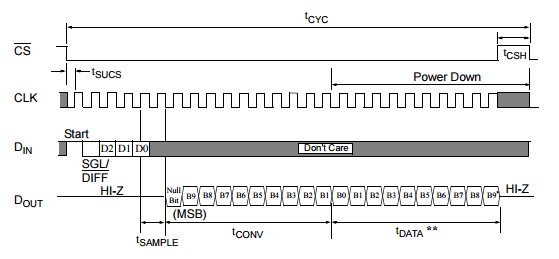
\includegraphics[width=\linewidth]{images/timing}
	\caption{Diagram showing the timings of a single communication.}
	\label{fig:timing}
\end{figure}

The entire communication process done to read a single conversion is depicted in figure \ref{fig:timing}. As can be seen, when \cs goes low, \din receives the five init bits. The sample and hold time is passed and a NULL bit followed by the result of the conversion is output on \dout. Throughout the period t$_\text{data}$ the chip is powering down and \dout reaches a high impedance state.
\subsection{Implementation of communication}
The communication between the MPC3008 and the FPGA is implemented as a VHDL component named ADC. 
The communication is implemented based on the timing diagram as showed in \ref{fig:timing}.  

\begin{figure}[h!]
	\centering
	\centerline{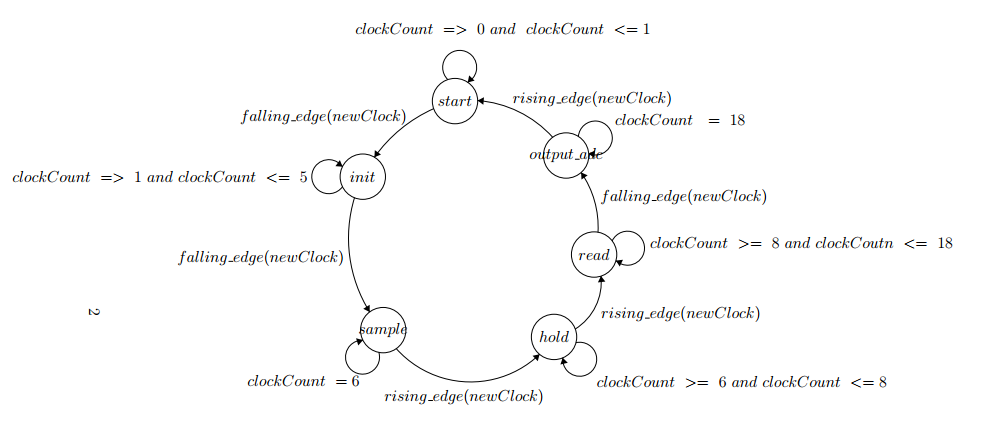
\includegraphics[width=18cm]{images/statemachine}}
	\caption{Program flow of the ADC component.}
	\label{fig:statemachine}
\end{figure}

As the MCP3008 operates at a clock frequency lower than what the FPGA provides. 
A process named \texttt{prescaler01} is designed to downscale the 50MHz external clock to the 3.57MHz required by the ADC. 
The downscaled clock is routed to \texttt{newClock}.


The process \texttt{ADC\_states}, increments \texttt{clockCount} for each rising edge on \texttt{newClock}.
This process detects both the falling and rising edges of \texttt{newClock}.

The progression of the state machine is based on the value of \texttt{clockCount}. 
This progression can be seen in figure \ref{fig:statemachine} and is explained below.\\

When \texttt{clockCount} is:
\begin{itemize}
	\item \textbf{0-1:} on the \texttt{falling\_edge} of \texttt{newClock}, \cs is set high, \texttt{MOSI} is set low and \texttt{read\_adc} is set low, signalling that conversion is not yet complete.\\
	\item \textbf{1-5:}on the \texttt{falling\_edge} of \texttt{newClock}, \cs is set low and the init bits are transmitted on \texttt{MOSI}, MSB first.
	\item \textbf{6:} on the \texttt{falling\_edge} of \texttt{newClock}, \texttt{MOSI} is set low. At this state MCP3008 starts sample and hold.
	\item \textbf{6-8:} on the \texttt{falling\_edge} of \texttt{newClock}, \texttt{MOSI} is kept low while the conversion is running. At \texttt{clockCount}=8 the MCP3008 outputs the NULL bit.
	\item \textbf{8-18:} on the \texttt{falling\_edge} of \texttt{newClock}, all 10 bits of the conversion are shifted from \texttt{MISO} into RX, a \texttt{std\_logic\_vector} containing the result of the conversion.
	\item \textbf{18:} on the \texttt{falling\_edge} of \texttt{newClock}, \texttt{read\_adc} is set high, signalling that conversion is complete and the result is ready.
	\item \textbf{19:} on the \texttt{falling\_edge} of \texttt{newClock}, \texttt{clockCount} is reset and the process starts over.
\end{itemize}

The conversion itself takes up only 17 \texttt{rising\_edges}, however one \texttt{clockCount} is used to set \cs high  and one \texttt{clockCount} is used to make sure that it read the 10 bit value. 


%begin{figure}[htb]
%\centering
%\begin{tikzpicture}[font=\sffamily,>=triangle 45]
%  \node [shape=circuit] (item) at (0,0) {adc};
%  \draw [<-] (item.ina) node [anchor=west,labels] {} -- +(-1,0) node [anchor=east] {MISO};
%  \draw [->] (item.outa) node [anchor=east,labels] {} -- +(1,0) node [anchor=west] {MOSI};
%  \draw [->] (item.outb) node [anchor=east,labels] {} -- +(1,0) node [anchor=west] {CS};
%  \draw [->] (item.outc) node [anchor=east,labels] {} -- +(1,0) node [anchor=west] {SCLK};
%  \draw [<-] (item.inb) node [anchor=west,labels] {} -- +(-1,0) node [anchor=east] {CLK};
%  \draw [->] (item.outd) node [anchor=east,labels] {} -- +(1,0) node [anchor=west] {read\_adc};
%  \draw [<-] (item.inc) node [anchor=west,labels] {} -- +(-1,0) node [anchor=east] {start\_adc};
%  \draw [->] (item.oute) node [anchor=east,labels] {} -- +(1,0) node [anchor=west] {ADC\_value};
%\end{tikzpicture}
%\caption{Entity of adc}
%\end{figure}

\subsection{Logic Level Converters}
When supplied with 5V, the MCP3008 uses TTL for communication while the FPGA uses 3.3V CMOS. To protect the FPGA it is necessary to translate the logic high of TTL, $V_h=5V$, to logic high of CMOS, $V_h=3.3V$. In order to achieve this, a simple circuit was utilized. See figure \ref{circ:logiclevel}. 

\begin{figure}[h!]
	\centering
	\begin{circuitikz}
		\draw(0,0)
			 node[above]{V$_\text{TTL}$}
				to[short,o-] ++(0.5,0)
					to[R=$R_1$] ++(2,0) node[circ]{} coordinate(junc)
						to[short,i=$i_c$] ++(0,-1)
							 ++(0,-1) node[ground](){}
							 	to[zDo=$D_1$] ++(0,1)
					(junc) to[short,-o] ++(1,0) node[above]{V$_\text{CMOS}$}
	;\end{circuitikz}
	\caption{Uni-directional logic level converter.}
	\label{circ:logiclevel}
\end{figure}  

This circuit is a uni-directional logic level converter, LLC. It will only allow for TTL to be converted to CMOS, not opposite. Ideally a bi-directional LLC should be created. This was not possible due to time constraints.

The zener diode chosen to clamp the voltage is the BZX79C3V3 \cite{bzx79c3v3}. 
This diode has a breakdown voltage of 3.3V. 
The current required to fully open the diode, $i_c$ is given in the datasheet as I$_\text{z}=5$mA.
As long as the input impedance of the FPGA is very high compared to $R_1$ it is reasonable to assume that V$_\text{CMOS}$ is open circuit.
By this assumption: $$R_1=\frac{\text{V}_\text{TTL}-\text{V}_\text{CMOS}}{i_c}=340\Omega$$